\documentclass{beamer}


\usetheme{CambridgeUS}

\usepackage{amsmath}
\usepackage{adjustbox}
\usepackage{amsmath}
\usepackage{amssymb}
\usepackage{relsize}
\usepackage{graphicx}
\usepackage{verbatim}
\usepackage{hyperref}
\usepackage{relsize}
\usepackage{amsthm}

\usepackage{pgffor}%
\usepackage{geometry}
\usepackage{pdflscape}

\usepackage[utf8]{inputenc}
\usepackage[english]{babel}


\newtheorem{proposition}[theorem]{Proposition}
\newtheorem{assumption}[theorem]{Assumption}

\begin{document}

\begin{frame}
\title{Impacts of Taxes on Firm Entry Rates along State Borders}
\author{Kevin D. Duncan, Georgeanne M. Artz, Peter F. Orazem \thanks{This study was supported by a grant from the Charles Koch Foundation}}
\institute{Iowa State University}
\date{May 11th, 2016 \\ Econometric Seminar}
\maketitle
\end{frame}

\begin{frame}
\frametitle{Overview}
\begin{itemize}
\item Contribution
\item Variables of interest
\item The estimation strategy
\begin{itemize}
\item Sorting around the border
\item County matching procedure
\item Estimated equation
\item Additional covariates
\item Remaining problems
\end{itemize}
\item The estimated effect
\item Sensitivity analysis
\end{itemize}
\end{frame}

\begin{frame}
\frametitle{Our contribution}

\begin{itemize}
\item We use a larger array of top marginal tax rates than other papers in the literature
\begin{itemize}
\item Property, income, sales, corporate, capital gains, workers compensation, unemployment insurance
\end{itemize}
\item Papers traditionally use only a small subset of tax rates (e.g. income, corporate, sales), creating plausible omitted variable bias
\item Some papers further don't use a non-endogenous proxy for effective tax rate, and we argue top marginal tax rate is the second best without firm characteristics
\item The border discontinuity approach to this problem is not the novel contribution
\end{itemize}

\end{frame}


\begin{frame}
\frametitle{Variable of Interest}
\begin{itemize}
\item Want to estimate the impacts of a 1\% increase in each of our different tax rates on firm start up rates
\item Doesn't fit well into (L)ATE framework; firms sort over tax policy regimes, no unconfoundness
\item Conditional logit and poisson models of sorting over all counties feature endogeneity of tax policy with respect to firm entry rates
\item County-differencing strategy aims to control for policy endogeneity under a similar set of assumptions of sorting, while removing likelihood estimation ("Local sorting/entry model")
\item End up estimat\textit{ing}  how a 1\% increase in each of our different tax rates impacts \textit{relative} firm start up rates
\end{itemize}
\end{frame}

\begin{frame}
\frametitle{Sorting at the border}
\begin{itemize}
\item Firms have face linear profit as a function of tax, regulatory, and location specific parameters.
\item Firms enter into perfectly competitive markets, and so can only pick at best one period of arbitrage profits
\item Conditional on picking to enter into a market around a state border, firms enter into the side of the border with the higher expected profits
\item No matter what, the number of new firm start ups on either side of the border will never be almost random around with respect to the treatment (different tax rates)
\end{itemize}
\end{frame}

\begin{frame}
\frametitle{Sorting at the border}
\begin{itemize}
\item But do think of this as a sorting problem!
\item We control for endogeneity of tax policy to firm entry rates by taking the difference in log firm start ups on states on either side of a state border; morphs dependent variable into relative firm start up rates, e.g. linear probability model
\item As if we are pulling a random firm from those that have decided to enter into some market around the state border, and we estimate the relative probabilities of that firm choosing one side of the border over the other
\item Much simpler criteria for identification, in particular, regular OLS identification requirements
\end{itemize}
\end{frame}

\begin{frame}
\frametitle{Matching}

\begin{itemize}
\item We use the Census Bureau's County Adjacency File (CAF) to match counties. The CAF orders states alphabetically, with counties alphabetically listed within. Adjacent counties are given similar treatment (e.g. first alphabetically by state, then alphabetically by county name).
\item We assign the first column as "subject" counties, and the adjacent counties as "neighbors"
\item Match each county in the subject column with every neighbor that is in another state.
\item Repeat until we generated the first unique set of matches.
\end{itemize}
\end{frame}

\begin{frame}
\frametitle{Matching: Example from the CAF}
\begin{center}
\begin{tabular}{cc} 
 \hline
 "Baldwin County, AL"  01003 & "Monroe County, AL"  01099 \\ 
 "Baldwin County, AL"  01003 & "Washington County, AL"  01129  \\ 
 "Baldwin County, AL"  01003 & "Escambia County, FL"  12033  \\ 
 "Barbour County, AL"  01005 & "Russell County, AL"  01113\\
 "Barbour County, AL"  01005 & "Clay County, GA"  13061\\
 "Barbour County, AL"  01005 & "Quitman County, GA"  13239\\
 \hline
\end{tabular}
\end{center}
\end{frame}

\begin{frame}
\frametitle{Matching: Visual Example}
\begin{figure}[h]\label{rb}
    \centering
    \textbf{Example of Border Matching}
    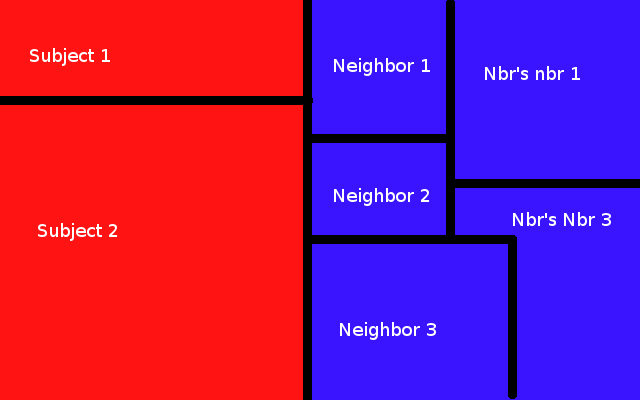
\includegraphics[scale = 0.35]{../../analysis/output/borders_temp.png}
    \caption{In this example Subject 1 would be only matched to Neighbor 1, while "Subject 2" would be paired with Neighbor 1-3. Similarly, when we broaden the bandwidth, Subject 1 would be matched with Nbr's Nbr 1, while Subject 2 would be paired with Nbr's Nbr 1 and 2.}
\end{figure}
\end{frame}

\begin{frame}
\frametitle{Estimating Equation}
\begin{itemize}
\item Imagine that we can approximate the log number of firms that enter into a county $i$ in a state $j$ in time $t$ by the equation
$$\ln(n_{ijt}) = X_{it}\gamma + X_{jt}\beta + e_{ijt}$$
\item Where $X_{it}$ are location specific effects, $X_{jt}$ are state specific effects, and $e_{ijt}$ is a composite shock term
\item Break up $e_{ijt}$ into three components, where we are given a countable collection of markets $g = 1,...,G$ that are sets of counties that may span different states.
$$e_{ijt} = \epsilon_{t} + \epsilon_{gt}+\epsilon_{ijt}$$
where $\epsilon_{t}$ is shared across all counties in all states, $\epsilon_{gt}$ is shared across all counties in a particular market, and $\epsilon_{ijt}$ is a true idiosyncratic error.
\item We want to estimate $\beta$.
\end{itemize}
\end{frame}

\begin{frame}
\frametitle{Estimating Equation}
\begin{itemize}
\item States may respond to both macroeconomic shocks along with federal governments, as well as market shocks that cover large areas of their territory. i.e. $\mathrm{E}(X_{jt}'e_{t}) \neq 0, \mathrm{E}(X_{jt}'e_{gt}) \neq 0$.
\item Differencing between "small enough" areas on either side of the border controls for this endogeneity and allows us to estimate a differenced equation of the form,

$$\ln(n_{ijt})-\ln(n_{i'j't}) = (X_{jt}-X_{j't})\beta + \epsilon_{ijt}-\epsilon_{i'j't}$$

\item Estimate with POLS and clustered standard errors at the state-pair level
\end{itemize}
\end{frame}

\begin{frame}
\frametitle{Additional Covariates}

\begin{itemize}
\item log state spending per capita on infrastructure, education, and welfare
\item optional state controls: real fuel price, percent unionized, percent manufacturing, percent high school education, population density
\item optional scaled geographic amenities: percent water, January sunlight, January temperature, July temperature, July humidity, topology score
\item State-pair specific fixed effects
\end{itemize}
\end{frame}

\begin{frame}
\frametitle{Remaining Problems}
\begin{itemize}
\item Properly capturing the relevant sorting variables along the border
\begin{itemize}
\item No measure of county level agglomeration economies in the paper to date
\item Some counties are quite large, and no ability to create effective methods to control for this
\end{itemize}
\item Omitted variable bias on not having county level tax and expenditure data
\begin{itemize}
\item Recent articles show that counties should optimally try and counteract the state level tax differential
\item This shrinks results towards zero
\end{itemize}
\item We cannot differentiate between pure new firms, firms that are part of chains that open up on both sides of the border, and firms that shut down on one side to open up on the other.
\end{itemize}
\end{frame}




\begin{frame}
\frametitle{The Estimated Effect}
\begin{table}[!htbp] \centering 
  \tiny
  \caption{Regression Discontinuity Models for  Total Firm Births} 
  \label{--rd} 
  {\tiny\renewcommand{\arraystretch}{.8}
\resizebox{!}{.25\paperheight}{%
\begin{tabular}{@{\extracolsep{5pt}}lcc} 
\\[-1.8ex]\hline 
\hline \\[-1.8ex] 
 & \multicolumn{2}{c}{\textit{births ratio}} \\ 
\cline{2-3} 
\hline \\[-1.8ex] 
  Property Tax Difference & $-$0.371$^{**}$ & $-$0.297$^{**}$ \\ 
  & (0.147) & (0.150) \\ 
  Income Tax Difference & $-$0.085$^{***}$ & $-$0.075$^{***}$ \\ 
  & (0.026) & (0.026)  \\ 
  Capital Gains Tax Difference  & 0.008 & 0.020 \\ 
  & (0.023) & (0.024) \\ 
  Sales Tax Difference & $-$0.101$^{***}$ & $-$0.087$^{***}$ \\ 
  & (0.030) & (0.032) \\ 
  Corp Tax Difference & 0.018 & 0.011  \\ 
  & (0.018) & (0.019) \\ 
  Workers Comp Tax Difference & 0.090 & 0.051 \\ 
  & (0.108) & (0.105) \\ 
  Unemp. Tax Difference & 0.012 & $-$0.006 \\ 
  & (0.036) & (0.038) \\ 
 \hline \\[-1.8ex] 
log expend & yes & yes \\
state controls  & yes & no\\ 
amenities & no & no \\
fixed effects & no & no \\
joint significance & yes & no \\
\hline \\[-1.8ex] 
\hline 
\hline \\[-1.8ex] 
Observations & 13,115 & 13,115 \\ 
G & 117 & 117 \\
R$^{2}$ & 0.056 &  0.037 \\ 
\hline 
\end{tabular}}}
\end{table} 
\end{frame}

\begin{frame}
\frametitle{Sensitivity Analysis}
\begin{itemize}
\item Not impose equality of the estimated effect on each side of the border
\item States that share reciprocal agreements
\item Sliding scale of urban v rural areas
\item Fixed effects for each state
\item Cross-sectional analysis for each year
\item Subsample estimates for 2-digit NAICS sectors
\item Extend the distance between each matched pair
\end{itemize}
\end{frame}

\begin{frame}

Thank you!

\end{frame}

\end{document}